\batchmode
\documentclass[a4paper]{book}
\usepackage{makeidx}
\usepackage{graphicx}
\usepackage{multicol}
\usepackage{float}
\usepackage{listings}
\usepackage{color}
\usepackage{ifthen}
\usepackage[table]{xcolor}
\usepackage{textcomp}
\usepackage{alltt}
\usepackage[utf8]{inputenc}
\usepackage{mathptmx}
\usepackage[scaled=.90]{helvet}
\usepackage{courier}
\usepackage{sectsty}
\usepackage[titles]{tocloft}
\usepackage{doxygen}
\lstset{language=C++,inputencoding=utf8,basicstyle=\footnotesize,breaklines=true,breakatwhitespace=true,tabsize=8,numbers=left }
\makeindex
\setcounter{tocdepth}{3}
\renewcommand{\footrulewidth}{0.4pt}
\renewcommand{\familydefault}{\sfdefault}
\begin{document}
\begin{titlepage}
\vspace*{7cm}
\begin{center}
{\Large teleop\_\-source\_\-joystick }\\
\vspace*{1cm}
{\large Generated by Doxygen 1.7.4}\\
\vspace*{0.5cm}
{\small Wed Feb 15 2012 22:36:51}\\
\end{center}
\end{titlepage}
\clearemptydoublepage
\pagenumbering{roman}
\tableofcontents
\clearemptydoublepage
\pagenumbering{arabic}
\chapter{Main Page}
\label{index}\input{index}
\chapter{Namespace Index}
\section{Namespace List}
Here is a list of all namespaces with brief descriptions:\begin{DoxyCompactList}
\item\contentsline{section}{{\bf ros} }{\pageref{namespaceros}}{}
\item\contentsline{section}{{\bf ros::message\_\-operations} }{\pageref{namespaceros_1_1message__operations}}{}
\item\contentsline{section}{{\bf ros::message\_\-traits} }{\pageref{namespaceros_1_1message__traits}}{}
\item\contentsline{section}{{\bf ros::serialization} }{\pageref{namespaceros_1_1serialization}}{}
\item\contentsline{section}{{\bf teleop\_\-msgs} }{\pageref{namespaceteleop__msgs}}{}
\item\contentsline{section}{{\bf teleop\_\-msgs::msg} }{\pageref{namespaceteleop__msgs_1_1msg}}{}
\item\contentsline{section}{{\bf teleop\_\-msgs::msg::\_\-Axis} }{\pageref{namespaceteleop__msgs_1_1msg_1_1__Axis}}{}
\item\contentsline{section}{{\bf teleop\_\-msgs::msg::\_\-Button} }{\pageref{namespaceteleop__msgs_1_1msg_1_1__Button}}{}
\item\contentsline{section}{{\bf teleop\_\-msgs::msg::\_\-State} }{\pageref{namespaceteleop__msgs_1_1msg_1_1__State}}{}
\end{DoxyCompactList}

\chapter{Class Index}
\section{Class List}
Here are the classes, structs, unions and interfaces with brief descriptions:\begin{DoxyCompactList}
\item\contentsline{section}{{\bf teleop::TeleopAxis} }{\pageref{structteleop_1_1TeleopAxis}}{}
\item\contentsline{section}{{\bf teleop::TeleopButton} }{\pageref{structteleop_1_1TeleopButton}}{}
\item\contentsline{section}{{\bf teleop::TeleopSource} }{\pageref{classteleop_1_1TeleopSource}}{}
\item\contentsline{section}{{\bf teleop::TeleopSourceAdapter} }{\pageref{classteleop_1_1TeleopSourceAdapter}}{}
\item\contentsline{section}{{\bf teleop::TeleopSourceAdapter::TeleopSourceAdapterCallback} }{\pageref{classteleop_1_1TeleopSourceAdapter_1_1TeleopSourceAdapterCallback}}{}
\item\contentsline{section}{{\bf teleop::TeleopState} }{\pageref{structteleop_1_1TeleopState}}{}
\end{DoxyCompactList}

\chapter{File Index}
\section{File List}
Here is a list of all files with brief descriptions:\begin{DoxyCompactList}
\item\contentsline{section}{/home/klc/Code/github.com/teleop/teleop\_\-source\_\-keyboard/include/{\bf teleop\_\-source\_\-keyboard.hpp} }{\pageref{teleop__source__keyboard_8hpp}}{}
\item\contentsline{section}{/home/klc/Code/github.com/teleop/teleop\_\-source\_\-keyboard/src/{\bf teleop\_\-source\_\-keyboard.cpp} }{\pageref{teleop__source__keyboard_8cpp}}{}
\end{DoxyCompactList}

\chapter{Namespace Documentation}
\section{teleop Namespace Reference}
\label{namespaceteleop}\index{teleop@{teleop}}
\subsection*{Classes}
\begin{DoxyCompactItemize}
\item 
class {\bf TeleopSourceJoystick}
\end{DoxyCompactItemize}

\chapter{Class Documentation}
\section{teleop::TeleopSourceJoystick Class Reference}
\label{classteleop_1_1TeleopSourceJoystick}\index{teleop::TeleopSourceJoystick@{teleop::TeleopSourceJoystick}}


{\ttfamily \#include $<$teleop\_\-source\_\-joystick.hpp$>$}

\subsection*{Public Member Functions}
\begin{DoxyCompactItemize}
\item 
std::string {\bf getDevice} ()
\item 
std::string {\bf getJoystickName} ()
\item 
virtual bool {\bf init} ()
\item 
virtual bool {\bf listen} (unsigned int listenTimeout, TeleopState $\ast$const teleopState, bool $\ast$updated)
\item 
bool {\bf setDevice} (std::string device)
\item 
virtual bool {\bf shutdown} ()
\item 
{\bf TeleopSourceJoystick} ()
\item 
{\bf $\sim$TeleopSourceJoystick} ()
\end{DoxyCompactItemize}
\subsection*{Static Public Member Functions}
\begin{DoxyCompactItemize}
\item 
static std::string {\bf getDefaultDevice} ()
\end{DoxyCompactItemize}
\subsection*{Private Member Functions}
\begin{DoxyCompactItemize}
\item 
bool {\bf handleEvent} (const js\_\-event $\ast$const event, TeleopState $\ast$const teleopState, bool $\ast$updated)
\end{DoxyCompactItemize}
\subsection*{Static Private Member Functions}
\begin{DoxyCompactItemize}
\item 
static TeleopAxisType {\bf axisDriverTypeToTeleopType} (\_\-\_\-u8 axisType)
\item 
static TeleopAxisValue {\bf axisDriverValueToTeleopValue} (\_\-\_\-s16 axisValue)
\item 
static TeleopButtonType {\bf buttonDriverTypeToTeleopType} (\_\-\_\-u16 buttonType)
\item 
static TeleopButtonValue {\bf buttonDriverValueToTeleopValue} (\_\-\_\-s16 buttonValue)
\end{DoxyCompactItemize}
\subsection*{Private Attributes}
\begin{DoxyCompactItemize}
\item 
\_\-\_\-u8 {\bf mAxisMap} [ABS\_\-CNT]
\item 
\_\-\_\-u16 {\bf mButtonMap} [KEY\_\-MAX-\/BTN\_\-MISC+1]
\item 
std::string {\bf mDevice}
\item 
int {\bf mFileDescriptor}
\item 
bool {\bf mIsInitialised}
\item 
std::string {\bf mJoystickName}
\item 
boost::recursive\_\-mutex {\bf mMemberMutex}
\item 
\_\-\_\-u8 {\bf mNumAxes}
\item 
\_\-\_\-u8 {\bf mNumButtons}
\end{DoxyCompactItemize}


\subsection{Detailed Description}
This class implements a joystick teleop source using the Linux kernel joystick driver. 

Definition at line 67 of file teleop\_\-source\_\-joystick.hpp.



\subsection{Constructor \& Destructor Documentation}
\index{teleop::TeleopSourceJoystick@{teleop::TeleopSourceJoystick}!TeleopSourceJoystick@{TeleopSourceJoystick}}
\index{TeleopSourceJoystick@{TeleopSourceJoystick}!teleop::TeleopSourceJoystick@{teleop::TeleopSourceJoystick}}
\subsubsection[{TeleopSourceJoystick}]{\setlength{\rightskip}{0pt plus 5cm}teleop::TeleopSourceJoystick::TeleopSourceJoystick (
\begin{DoxyParamCaption}
{}
\end{DoxyParamCaption}
)}\label{classteleop_1_1TeleopSourceJoystick_a752cf0ad7022c1ec423ee01c9eb0ba7c}
Constructor. 

Definition at line 78 of file teleop\_\-source\_\-joystick.cpp.

\index{teleop::TeleopSourceJoystick@{teleop::TeleopSourceJoystick}!$\sim$TeleopSourceJoystick@{$\sim$TeleopSourceJoystick}}
\index{$\sim$TeleopSourceJoystick@{$\sim$TeleopSourceJoystick}!teleop::TeleopSourceJoystick@{teleop::TeleopSourceJoystick}}
\subsubsection[{$\sim$TeleopSourceJoystick}]{\setlength{\rightskip}{0pt plus 5cm}teleop::TeleopSourceJoystick::$\sim$TeleopSourceJoystick (
\begin{DoxyParamCaption}
{}
\end{DoxyParamCaption}
)}\label{classteleop_1_1TeleopSourceJoystick_a40d3b922cf1b425438fbcbf20cec2ce6}
Destructor. 

Definition at line 94 of file teleop\_\-source\_\-joystick.cpp.



\subsection{Member Function Documentation}
\index{teleop::TeleopSourceJoystick@{teleop::TeleopSourceJoystick}!axisDriverTypeToTeleopType@{axisDriverTypeToTeleopType}}
\index{axisDriverTypeToTeleopType@{axisDriverTypeToTeleopType}!teleop::TeleopSourceJoystick@{teleop::TeleopSourceJoystick}}
\subsubsection[{axisDriverTypeToTeleopType}]{\setlength{\rightskip}{0pt plus 5cm}TeleopAxisType teleop::TeleopSourceJoystick::axisDriverTypeToTeleopType (
\begin{DoxyParamCaption}
\item[{\_\-\_\-u8}]{axisType}
\end{DoxyParamCaption}
)\hspace{0.3cm}{\ttfamily  [static, private]}}\label{classteleop_1_1TeleopSourceJoystick_abfbd4b45c058dff074394c8ca7db5aef}
Convert driver axis type to teleop axis type.


\begin{DoxyParams}{Parameters}
{\em axisType} & [in] -\/ driver axis type to convert\\
\hline
\end{DoxyParams}
\begin{DoxyReturn}{Returns}
teleop axis type 
\end{DoxyReturn}


Definition at line 409 of file teleop\_\-source\_\-joystick.cpp.

\index{teleop::TeleopSourceJoystick@{teleop::TeleopSourceJoystick}!axisDriverValueToTeleopValue@{axisDriverValueToTeleopValue}}
\index{axisDriverValueToTeleopValue@{axisDriverValueToTeleopValue}!teleop::TeleopSourceJoystick@{teleop::TeleopSourceJoystick}}
\subsubsection[{axisDriverValueToTeleopValue}]{\setlength{\rightskip}{0pt plus 5cm}TeleopAxisValue teleop::TeleopSourceJoystick::axisDriverValueToTeleopValue (
\begin{DoxyParamCaption}
\item[{\_\-\_\-s16}]{axisValue}
\end{DoxyParamCaption}
)\hspace{0.3cm}{\ttfamily  [static, private]}}\label{classteleop_1_1TeleopSourceJoystick_a7f2308579be85beec4b57deff4856fbb}
Convert driver axis value to teleop axis value.


\begin{DoxyParams}{Parameters}
{\em axisValue} & [in] -\/ driver axis value to convert\\
\hline
\end{DoxyParams}
\begin{DoxyReturn}{Returns}
teleop axis value 
\end{DoxyReturn}


Definition at line 401 of file teleop\_\-source\_\-joystick.cpp.

\index{teleop::TeleopSourceJoystick@{teleop::TeleopSourceJoystick}!buttonDriverTypeToTeleopType@{buttonDriverTypeToTeleopType}}
\index{buttonDriverTypeToTeleopType@{buttonDriverTypeToTeleopType}!teleop::TeleopSourceJoystick@{teleop::TeleopSourceJoystick}}
\subsubsection[{buttonDriverTypeToTeleopType}]{\setlength{\rightskip}{0pt plus 5cm}TeleopButtonType teleop::TeleopSourceJoystick::buttonDriverTypeToTeleopType (
\begin{DoxyParamCaption}
\item[{\_\-\_\-u16}]{buttonType}
\end{DoxyParamCaption}
)\hspace{0.3cm}{\ttfamily  [static, private]}}\label{classteleop_1_1TeleopSourceJoystick_a364550301c3f48ba1e30f1a2269bca64}
Convert driver button type to teleop button type.


\begin{DoxyParams}{Parameters}
{\em buttonType} & [in] -\/ driver button type to convert\\
\hline
\end{DoxyParams}
\begin{DoxyReturn}{Returns}
teleop button type 
\end{DoxyReturn}


Definition at line 436 of file teleop\_\-source\_\-joystick.cpp.

\index{teleop::TeleopSourceJoystick@{teleop::TeleopSourceJoystick}!buttonDriverValueToTeleopValue@{buttonDriverValueToTeleopValue}}
\index{buttonDriverValueToTeleopValue@{buttonDriverValueToTeleopValue}!teleop::TeleopSourceJoystick@{teleop::TeleopSourceJoystick}}
\subsubsection[{buttonDriverValueToTeleopValue}]{\setlength{\rightskip}{0pt plus 5cm}TeleopButtonValue teleop::TeleopSourceJoystick::buttonDriverValueToTeleopValue (
\begin{DoxyParamCaption}
\item[{\_\-\_\-s16}]{buttonValue}
\end{DoxyParamCaption}
)\hspace{0.3cm}{\ttfamily  [static, private]}}\label{classteleop_1_1TeleopSourceJoystick_a3def96790275bb1aed61a92ad0e62155}
Convert driver button value to teleop button value.


\begin{DoxyParams}{Parameters}
{\em buttonValue} & [in] -\/ driver button value to convert\\
\hline
\end{DoxyParams}
\begin{DoxyReturn}{Returns}
teleop button value 
\end{DoxyReturn}


Definition at line 405 of file teleop\_\-source\_\-joystick.cpp.

\index{teleop::TeleopSourceJoystick@{teleop::TeleopSourceJoystick}!getDefaultDevice@{getDefaultDevice}}
\index{getDefaultDevice@{getDefaultDevice}!teleop::TeleopSourceJoystick@{teleop::TeleopSourceJoystick}}
\subsubsection[{getDefaultDevice}]{\setlength{\rightskip}{0pt plus 5cm}std::string teleop::TeleopSourceJoystick::getDefaultDevice (
\begin{DoxyParamCaption}
{}
\end{DoxyParamCaption}
)\hspace{0.3cm}{\ttfamily  [static]}}\label{classteleop_1_1TeleopSourceJoystick_a1dd7f20235ea6ed665ff88898dadf687}
Get default device.

\begin{DoxyReturn}{Returns}
default device 
\end{DoxyReturn}


Definition at line 463 of file teleop\_\-source\_\-joystick.cpp.

\index{teleop::TeleopSourceJoystick@{teleop::TeleopSourceJoystick}!getDevice@{getDevice}}
\index{getDevice@{getDevice}!teleop::TeleopSourceJoystick@{teleop::TeleopSourceJoystick}}
\subsubsection[{getDevice}]{\setlength{\rightskip}{0pt plus 5cm}std::string teleop::TeleopSourceJoystick::getDevice (
\begin{DoxyParamCaption}
{}
\end{DoxyParamCaption}
)}\label{classteleop_1_1TeleopSourceJoystick_ab9cd0ec812ddb003f6a48cfca0902200}
Get device.

\begin{DoxyReturn}{Returns}
device 
\end{DoxyReturn}


Definition at line 112 of file teleop\_\-source\_\-joystick.cpp.

\index{teleop::TeleopSourceJoystick@{teleop::TeleopSourceJoystick}!getJoystickName@{getJoystickName}}
\index{getJoystickName@{getJoystickName}!teleop::TeleopSourceJoystick@{teleop::TeleopSourceJoystick}}
\subsubsection[{getJoystickName}]{\setlength{\rightskip}{0pt plus 5cm}std::string teleop::TeleopSourceJoystick::getJoystickName (
\begin{DoxyParamCaption}
{}
\end{DoxyParamCaption}
)}\label{classteleop_1_1TeleopSourceJoystick_a9837bc5a677e9ac8bd0f42b3c492045f}
Get joystick name.

\begin{DoxyReturn}{Returns}
joystick name 
\end{DoxyReturn}


Definition at line 120 of file teleop\_\-source\_\-joystick.cpp.

\index{teleop::TeleopSourceJoystick@{teleop::TeleopSourceJoystick}!handleEvent@{handleEvent}}
\index{handleEvent@{handleEvent}!teleop::TeleopSourceJoystick@{teleop::TeleopSourceJoystick}}
\subsubsection[{handleEvent}]{\setlength{\rightskip}{0pt plus 5cm}bool teleop::TeleopSourceJoystick::handleEvent (
\begin{DoxyParamCaption}
\item[{const js\_\-event $\ast$const}]{event, }
\item[{TeleopState $\ast$const}]{teleopState, }
\item[{bool $\ast$}]{updated}
\end{DoxyParamCaption}
)\hspace{0.3cm}{\ttfamily  [private]}}\label{classteleop_1_1TeleopSourceJoystick_a48426a7e8588f64485a12d6cafd8cc60}
Handle a given event.


\begin{DoxyParams}{Parameters}
{\em event} & [in] -\/ event to handle \\
\hline
{\em teleopState} & [in/out] -\/ the current teleop state, to be updated \\
\hline
{\em updated} & [in/out] -\/ true if teleop state was updated\\
\hline
\end{DoxyParams}
\begin{DoxyReturn}{Returns}
true on success 
\end{DoxyReturn}


Definition at line 339 of file teleop\_\-source\_\-joystick.cpp.

\index{teleop::TeleopSourceJoystick@{teleop::TeleopSourceJoystick}!init@{init}}
\index{init@{init}!teleop::TeleopSourceJoystick@{teleop::TeleopSourceJoystick}}
\subsubsection[{init}]{\setlength{\rightskip}{0pt plus 5cm}bool teleop::TeleopSourceJoystick::init (
\begin{DoxyParamCaption}
{}
\end{DoxyParamCaption}
)\hspace{0.3cm}{\ttfamily  [virtual]}}\label{classteleop_1_1TeleopSourceJoystick_a3396ee936f2f73bbb52502a3d06acdaa}
Override virtual method from parent. 

Definition at line 128 of file teleop\_\-source\_\-joystick.cpp.

\index{teleop::TeleopSourceJoystick@{teleop::TeleopSourceJoystick}!listen@{listen}}
\index{listen@{listen}!teleop::TeleopSourceJoystick@{teleop::TeleopSourceJoystick}}
\subsubsection[{listen}]{\setlength{\rightskip}{0pt plus 5cm}bool teleop::TeleopSourceJoystick::listen (
\begin{DoxyParamCaption}
\item[{unsigned int}]{listenTimeout, }
\item[{TeleopState $\ast$const}]{teleopState, }
\item[{bool $\ast$}]{updated}
\end{DoxyParamCaption}
)\hspace{0.3cm}{\ttfamily  [virtual]}}\label{classteleop_1_1TeleopSourceJoystick_ae224a140f250cab4873d3d8e4c497069}
Override virtual method from parent. 

Definition at line 228 of file teleop\_\-source\_\-joystick.cpp.

\index{teleop::TeleopSourceJoystick@{teleop::TeleopSourceJoystick}!setDevice@{setDevice}}
\index{setDevice@{setDevice}!teleop::TeleopSourceJoystick@{teleop::TeleopSourceJoystick}}
\subsubsection[{setDevice}]{\setlength{\rightskip}{0pt plus 5cm}bool teleop::TeleopSourceJoystick::setDevice (
\begin{DoxyParamCaption}
\item[{std::string}]{device}
\end{DoxyParamCaption}
)}\label{classteleop_1_1TeleopSourceJoystick_a32eefaad1dda8c559b1abcb301267eba}
Set device. Should only be called before \doxyref{init()}{p.}{classteleop_1_1TeleopSourceJoystick_a3396ee936f2f73bbb52502a3d06acdaa} or after \doxyref{shutdown()}{p.}{classteleop_1_1TeleopSourceJoystick_a6eef5c77c0da488ab6bf0d80c376dca0}.


\begin{DoxyParams}{Parameters}
{\em device} & -\/ device to set\\
\hline
\end{DoxyParams}
\begin{DoxyReturn}{Returns}
true on success 
\end{DoxyReturn}


Definition at line 101 of file teleop\_\-source\_\-joystick.cpp.

\index{teleop::TeleopSourceJoystick@{teleop::TeleopSourceJoystick}!shutdown@{shutdown}}
\index{shutdown@{shutdown}!teleop::TeleopSourceJoystick@{teleop::TeleopSourceJoystick}}
\subsubsection[{shutdown}]{\setlength{\rightskip}{0pt plus 5cm}bool teleop::TeleopSourceJoystick::shutdown (
\begin{DoxyParamCaption}
{}
\end{DoxyParamCaption}
)\hspace{0.3cm}{\ttfamily  [virtual]}}\label{classteleop_1_1TeleopSourceJoystick_a6eef5c77c0da488ab6bf0d80c376dca0}
Override virtual method from parent. 

Definition at line 310 of file teleop\_\-source\_\-joystick.cpp.



\subsection{Member Data Documentation}
\index{teleop::TeleopSourceJoystick@{teleop::TeleopSourceJoystick}!mAxisMap@{mAxisMap}}
\index{mAxisMap@{mAxisMap}!teleop::TeleopSourceJoystick@{teleop::TeleopSourceJoystick}}
\subsubsection[{mAxisMap}]{\setlength{\rightskip}{0pt plus 5cm}\_\-\_\-u8 {\bf teleop::TeleopSourceJoystick::mAxisMap}[ABS\_\-CNT]\hspace{0.3cm}{\ttfamily  [private]}}\label{classteleop_1_1TeleopSourceJoystick_ab7018820d3d62d5ef8d77528f3096444}
Axis type map from driver 

Definition at line 147 of file teleop\_\-source\_\-joystick.hpp.

\index{teleop::TeleopSourceJoystick@{teleop::TeleopSourceJoystick}!mButtonMap@{mButtonMap}}
\index{mButtonMap@{mButtonMap}!teleop::TeleopSourceJoystick@{teleop::TeleopSourceJoystick}}
\subsubsection[{mButtonMap}]{\setlength{\rightskip}{0pt plus 5cm}\_\-\_\-u16 {\bf teleop::TeleopSourceJoystick::mButtonMap}[KEY\_\-MAX-\/BTN\_\-MISC+1]\hspace{0.3cm}{\ttfamily  [private]}}\label{classteleop_1_1TeleopSourceJoystick_a40cab6d847daa209b36df0fc471a1cd8}
Button type map from driver 

Definition at line 153 of file teleop\_\-source\_\-joystick.hpp.

\index{teleop::TeleopSourceJoystick@{teleop::TeleopSourceJoystick}!mDevice@{mDevice}}
\index{mDevice@{mDevice}!teleop::TeleopSourceJoystick@{teleop::TeleopSourceJoystick}}
\subsubsection[{mDevice}]{\setlength{\rightskip}{0pt plus 5cm}std::string {\bf teleop::TeleopSourceJoystick::mDevice}\hspace{0.3cm}{\ttfamily  [private]}}\label{classteleop_1_1TeleopSourceJoystick_a4423b7cf74b8e40655277a7c98acc3be}
Device 

Definition at line 135 of file teleop\_\-source\_\-joystick.hpp.

\index{teleop::TeleopSourceJoystick@{teleop::TeleopSourceJoystick}!mFileDescriptor@{mFileDescriptor}}
\index{mFileDescriptor@{mFileDescriptor}!teleop::TeleopSourceJoystick@{teleop::TeleopSourceJoystick}}
\subsubsection[{mFileDescriptor}]{\setlength{\rightskip}{0pt plus 5cm}int {\bf teleop::TeleopSourceJoystick::mFileDescriptor}\hspace{0.3cm}{\ttfamily  [private]}}\label{classteleop_1_1TeleopSourceJoystick_a52cc674afb32309b1c7e5b4a7416d301}
File descriptor 

Definition at line 141 of file teleop\_\-source\_\-joystick.hpp.

\index{teleop::TeleopSourceJoystick@{teleop::TeleopSourceJoystick}!mIsInitialised@{mIsInitialised}}
\index{mIsInitialised@{mIsInitialised}!teleop::TeleopSourceJoystick@{teleop::TeleopSourceJoystick}}
\subsubsection[{mIsInitialised}]{\setlength{\rightskip}{0pt plus 5cm}bool {\bf teleop::TeleopSourceJoystick::mIsInitialised}\hspace{0.3cm}{\ttfamily  [private]}}\label{classteleop_1_1TeleopSourceJoystick_a13daf98aca315b4d35b11f253e57a299}
Flag indicating if we are prepared to listen 

Definition at line 132 of file teleop\_\-source\_\-joystick.hpp.

\index{teleop::TeleopSourceJoystick@{teleop::TeleopSourceJoystick}!mJoystickName@{mJoystickName}}
\index{mJoystickName@{mJoystickName}!teleop::TeleopSourceJoystick@{teleop::TeleopSourceJoystick}}
\subsubsection[{mJoystickName}]{\setlength{\rightskip}{0pt plus 5cm}std::string {\bf teleop::TeleopSourceJoystick::mJoystickName}\hspace{0.3cm}{\ttfamily  [private]}}\label{classteleop_1_1TeleopSourceJoystick_aaa1c80abaa5d2e3323260b2fadbcbc79}
Joystick name 

Definition at line 138 of file teleop\_\-source\_\-joystick.hpp.

\index{teleop::TeleopSourceJoystick@{teleop::TeleopSourceJoystick}!mMemberMutex@{mMemberMutex}}
\index{mMemberMutex@{mMemberMutex}!teleop::TeleopSourceJoystick@{teleop::TeleopSourceJoystick}}
\subsubsection[{mMemberMutex}]{\setlength{\rightskip}{0pt plus 5cm}boost::recursive\_\-mutex {\bf teleop::TeleopSourceJoystick::mMemberMutex}\hspace{0.3cm}{\ttfamily  [private]}}\label{classteleop_1_1TeleopSourceJoystick_a5d1ab902a193ff2a0c81af814489184c}
Mutex for protecting all members from multi-\/threaded access 

Definition at line 129 of file teleop\_\-source\_\-joystick.hpp.

\index{teleop::TeleopSourceJoystick@{teleop::TeleopSourceJoystick}!mNumAxes@{mNumAxes}}
\index{mNumAxes@{mNumAxes}!teleop::TeleopSourceJoystick@{teleop::TeleopSourceJoystick}}
\subsubsection[{mNumAxes}]{\setlength{\rightskip}{0pt plus 5cm}\_\-\_\-u8 {\bf teleop::TeleopSourceJoystick::mNumAxes}\hspace{0.3cm}{\ttfamily  [private]}}\label{classteleop_1_1TeleopSourceJoystick_af61f32af6e9ebf8df8d1ac3607ffa750}
Number of axes from driver 

Definition at line 144 of file teleop\_\-source\_\-joystick.hpp.

\index{teleop::TeleopSourceJoystick@{teleop::TeleopSourceJoystick}!mNumButtons@{mNumButtons}}
\index{mNumButtons@{mNumButtons}!teleop::TeleopSourceJoystick@{teleop::TeleopSourceJoystick}}
\subsubsection[{mNumButtons}]{\setlength{\rightskip}{0pt plus 5cm}\_\-\_\-u8 {\bf teleop::TeleopSourceJoystick::mNumButtons}\hspace{0.3cm}{\ttfamily  [private]}}\label{classteleop_1_1TeleopSourceJoystick_a46c70ceedbe92833016dc9b6cfe0278d}
Number of buttons from driver 

Definition at line 150 of file teleop\_\-source\_\-joystick.hpp.



The documentation for this class was generated from the following files:\begin{DoxyCompactItemize}
\item 
{\bf teleop\_\-source\_\-joystick.hpp}\item 
{\bf teleop\_\-source\_\-joystick.cpp}\end{DoxyCompactItemize}

\chapter{File Documentation}
\section{teleop\_\-source\_\-joystick.hpp File Reference}
\label{teleop__source__joystick_8hpp}\index{teleop\_\-source\_\-joystick.hpp@{teleop\_\-source\_\-joystick.hpp}}
{\ttfamily \#include $<$teleop\_\-common.hpp$>$}\par
{\ttfamily \#include $<$teleop\_\-source.hpp$>$}\par
{\ttfamily \#include $<$boost/thread.hpp$>$}\par
{\ttfamily \#include $<$linux/types.h$>$}\par
{\ttfamily \#include $<$linux/joystick.h$>$}\par
Include dependency graph for teleop\_\-source\_\-joystick.hpp:
\nopagebreak
\begin{figure}[H]
\begin{center}
\leavevmode
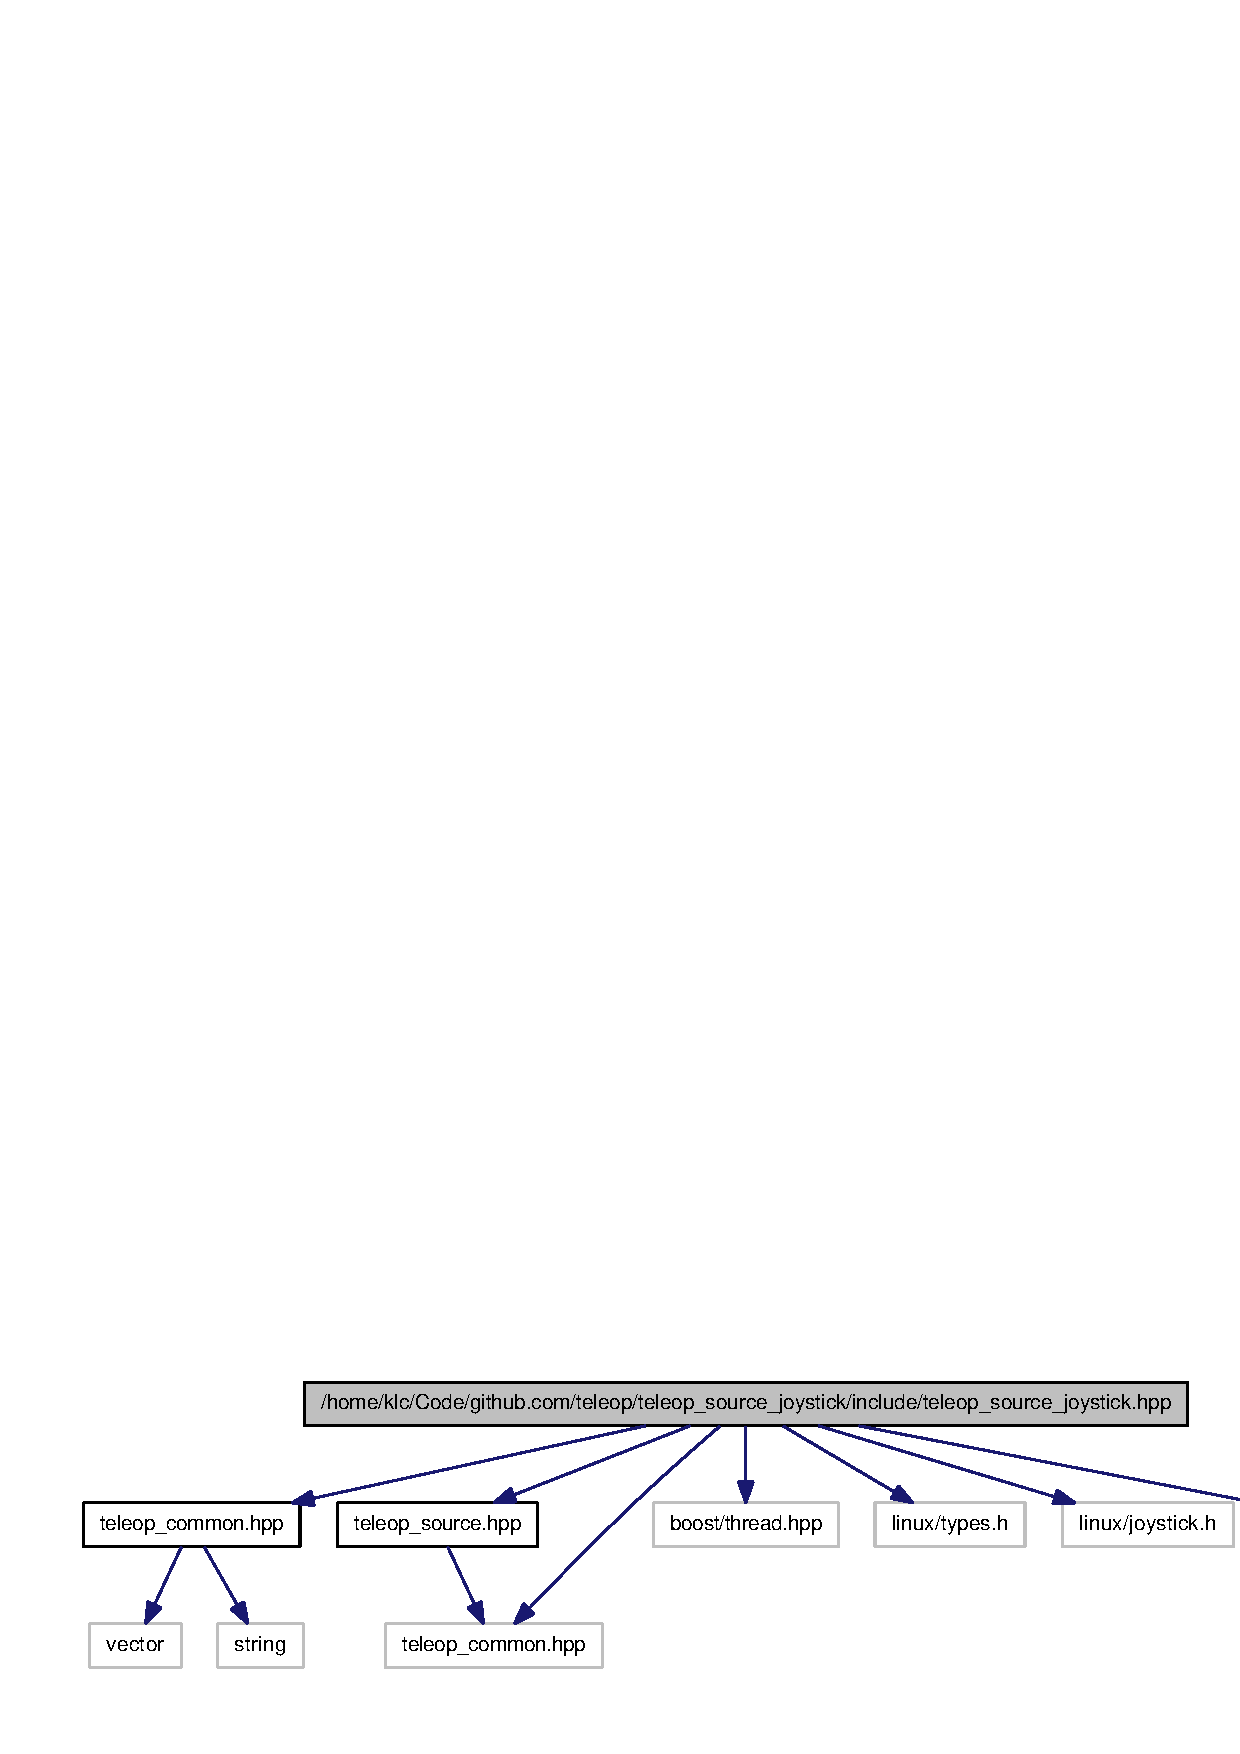
\includegraphics[width=400pt]{teleop__source__joystick_8hpp__incl}
\end{center}
\end{figure}
This graph shows which files directly or indirectly include this file:
\nopagebreak
\begin{figure}[H]
\begin{center}
\leavevmode
\includegraphics[width=178pt]{teleop__source__joystick_8hpp__dep__incl}
\end{center}
\end{figure}
\subsection*{Classes}
\begin{DoxyCompactItemize}
\item 
class {\bf teleop::TeleopSourceJoystick}
\end{DoxyCompactItemize}
\subsection*{Namespaces}
\begin{DoxyCompactItemize}
\item 
namespace {\bf teleop}
\end{DoxyCompactItemize}

\section{/home/klc/Code/github.com/teleop/teleop\_\-source\_\-joystick/mainpage.dox File Reference}
\label{mainpage_8dox}\index{/home/klc/Code/github.com/teleop/teleop\_\-source\_\-joystick/mainpage.dox@{/home/klc/Code/github.com/teleop/teleop\_\-source\_\-joystick/mainpage.dox}}

\section{teleop\_\-source\_\-joystick.cpp File Reference}
\label{teleop__source__joystick_8cpp}\index{teleop\_\-source\_\-joystick.cpp@{teleop\_\-source\_\-joystick.cpp}}
{\ttfamily \#include $<$teleop\_\-common.hpp$>$}\par
{\ttfamily \#include $<$teleop\_\-source.hpp$>$}\par
{\ttfamily \#include $<$teleop\_\-source\_\-joystick.hpp$>$}\par
{\ttfamily \#include $<$boost/thread.hpp$>$}\par
{\ttfamily \#include $<$linux/types.h$>$}\par
{\ttfamily \#include $<$linux/input.h$>$}\par
{\ttfamily \#include $<$linux/joystick.h$>$}\par
{\ttfamily \#include $<$sys/select.h$>$}\par
{\ttfamily \#include $<$unistd.h$>$}\par
{\ttfamily \#include $<$time.h$>$}\par
{\ttfamily \#include $<$fcntl.h$>$}\par
{\ttfamily \#include $<$stdio.h$>$}\par
{\ttfamily \#include $<$errno.h$>$}\par
Include dependency graph for teleop\_\-source\_\-joystick.cpp:
\nopagebreak
\begin{figure}[H]
\begin{center}
\leavevmode
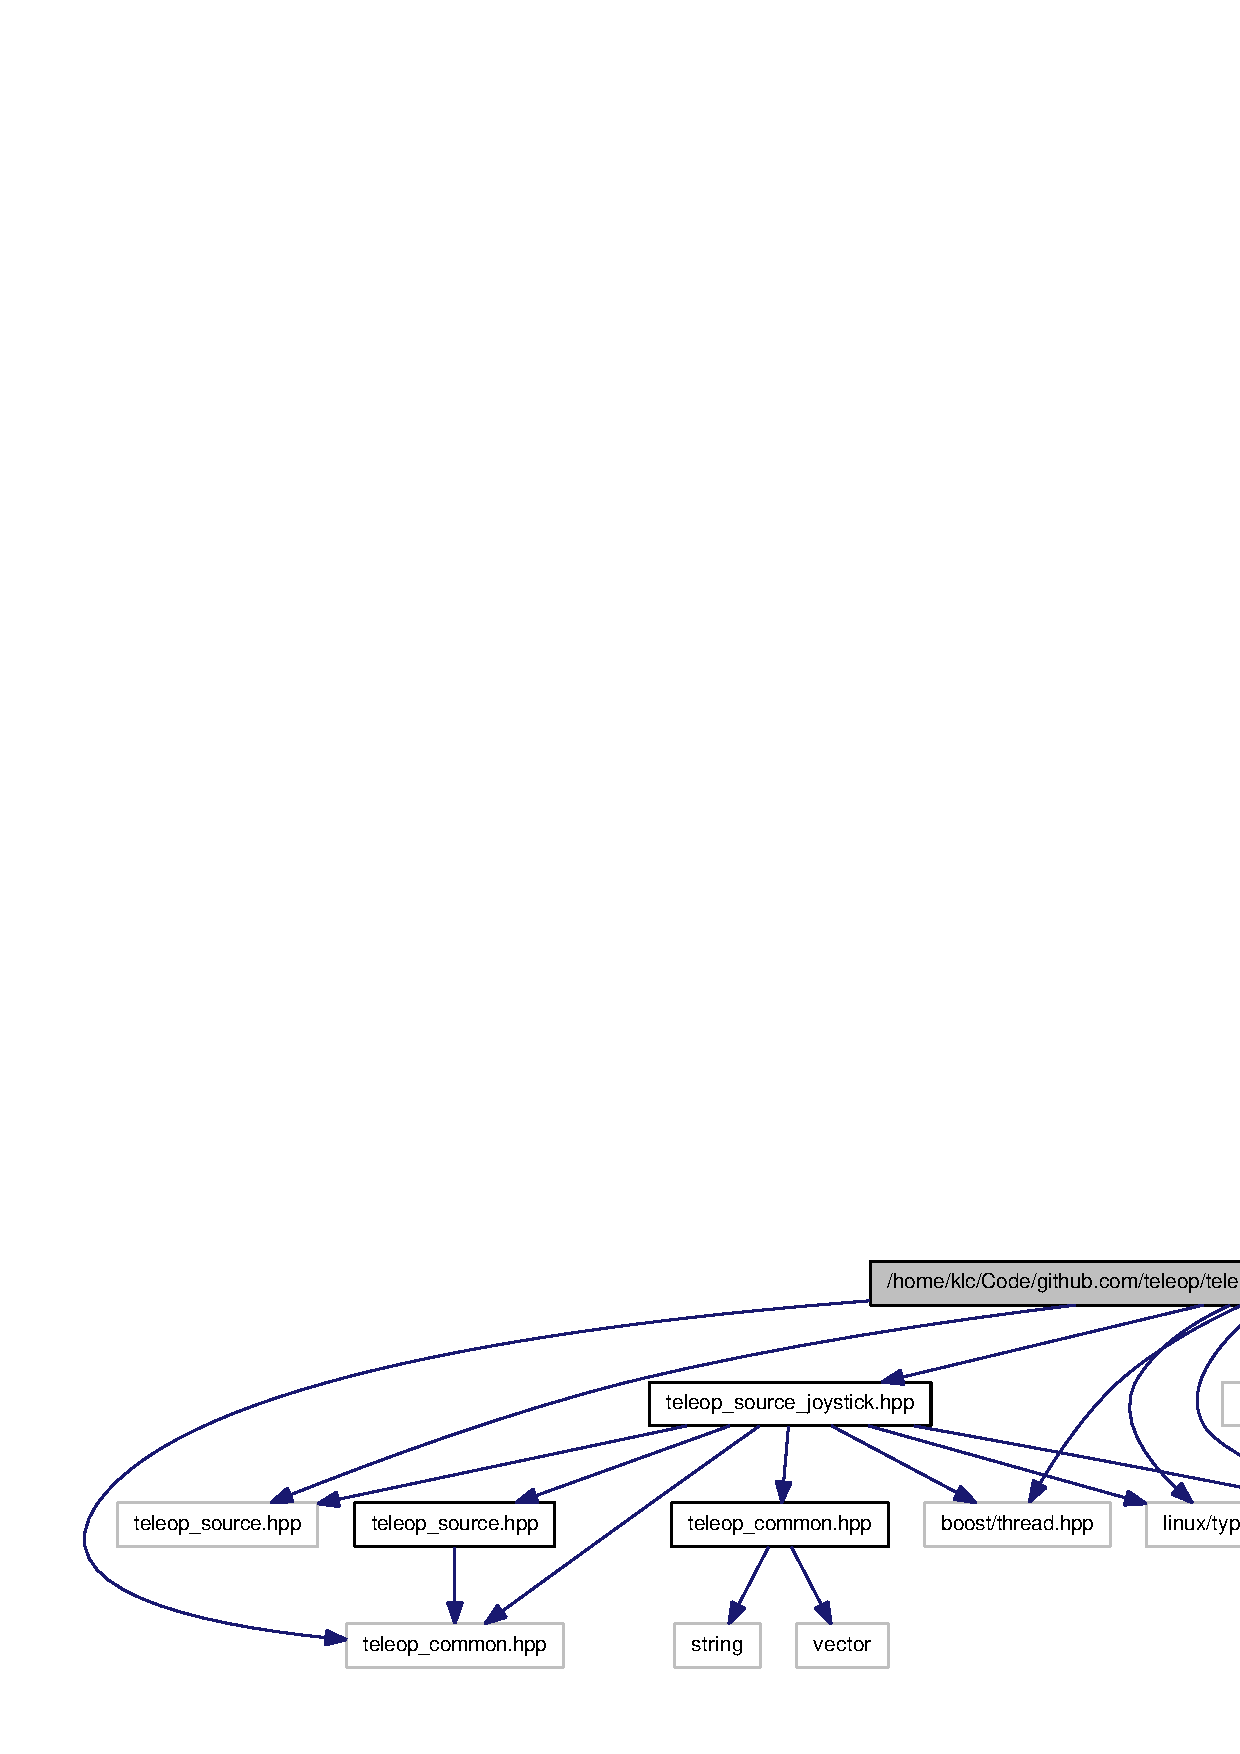
\includegraphics[width=400pt]{teleop__source__joystick_8cpp__incl}
\end{center}
\end{figure}
\subsection*{Namespaces}
\begin{DoxyCompactItemize}
\item 
namespace {\bf teleop}
\end{DoxyCompactItemize}

\printindex
\end{document}
